\documentclass[tikz]{standalone}
\usepackage{amsmath}
\usepackage{amssymb}
\usepackage{amsfonts}
\usepackage{tikz}
\usetikzlibrary{positioning, arrows.meta}

\thispagestyle{empty}
\begin{document}

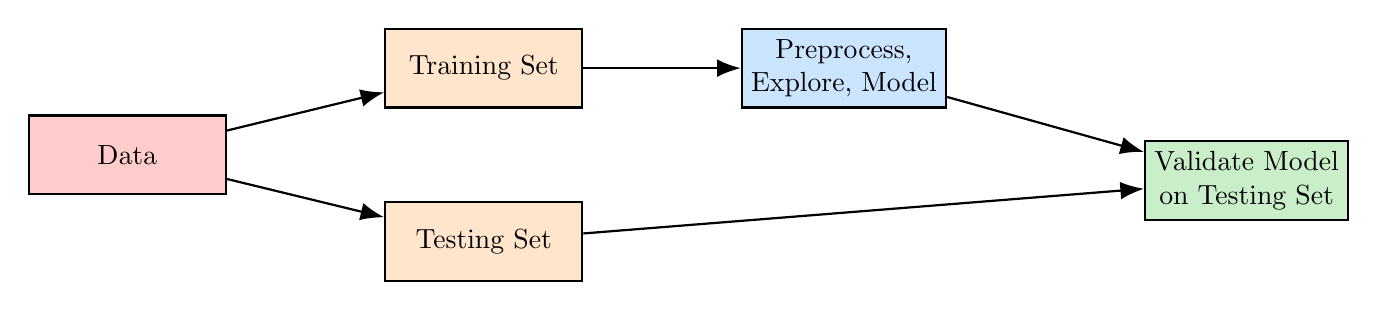
\begin{tikzpicture}[ node distance=1.5cm and 2cm,
box/.style={draw, thick, minimum width=2.5cm, minimum height=1cm, align=center},
arrow/.style={thick, -{Latex[length=3mm]}} ]

% Define colors
\definecolor{softred}{RGB}{255, 204, 204}
\definecolor{softorange}{RGB}{255, 229, 204}
\definecolor{softyellow}{RGB}{255, 255, 204}
\definecolor{softgreen}{RGB}{202, 238, 202}
\definecolor{softblue}{RGB}{204, 229, 255}

% Nodes
\node[box, fill=softred] (data) {Data};
\node[box, fill=softorange, right=of data, yshift=1.1cm] (train) {Training Set};
\node[box, fill=softorange, right=of data, yshift=-1.1cm] (test) {Testing Set};
\node[box, fill=softblue, right=of train] (process) {Preprocess,\\ Explore, Model};
\node[box, fill=softgreen, below right=0.4cm and 2.5cm of process] (validate) {Validate Model\\ on Testing Set};

% Arrows
\draw[arrow] (data) -- (train);
\draw[arrow] (data) -- (test);
\draw[arrow] (train) -- (process);
\draw[arrow] (process) -- (validate);
\draw[arrow] (test) -- (validate);

\end{tikzpicture}
\end{document}
